% !TeX spellcheck = en_US

\section{Problem 8}
ADALINE is a single-layer artificial neural network that can learn and adapt to non-linear relationships between inputs and outputs. \\
It consists of a single neuron with a linear activation function. Each input of the neuron has a corresponding weight,which is adapted during training to minimize the error between the network's output and the desired output. To adjust the weights the algorithm uses the learning rule α.
\vspace{0.3cm}

Suppose that we have the following three reference patterns and their targets:
\vspace{5mm}

\[
\begin{array}{ccc}
%	\centering
	\left\{ 
	p_1 = \left[
	\begin{array}{c}
		2 \\
		4
	\end{array}
	\right], t_1 = \left[26\right]
	\right\} & 
	\left\{ 
	p_2 = \left[
	\begin{array}{c}
		4 \\
		2
	\end{array}
	\right], t_2 = \left[26\right]
	\right\}
	&\left\{ 
	p_3 = \left[
	\begin{array}{c}
		-2 \\
		-2
	\end{array}
	\right], t_3 = \left[-26\right]
	\right\}
	
\end{array}
\]

\vspace{5mm}

The probability of vector p1 is $P_{1}= 0.20$, the probability of vector p2 is $P_{2}= 0.70$, and the probability of vector p3 is $P_{3}= 0.10$.


\subsection{Question a}
The number of inputs to an ADALINE network for each neural network is determined by the dimensionality of our data,not by the number of patterns we have. In our case, each pattern is a 2-dimensional vector. Therefore, our ADALINE network has two inputs, one for each dimension.\\
In an ADALINE network, the number of weights is equal to the number of inputs. In our case, we have two inputs. Thus, our neural network has two weights, one for each dimension of the input.\\
From theory, the output of an ADALINE network is a = purelin($W_{p}$+b).\\

So, the network diagram for the given ADALINE network with no bias that will be trained with  these patterns is shown in figure \ref{fig:prob8_adaline_draw}.\\

\begin{figure}[H]
	\centering
	\includesvg[width=0.7\textwidth]{../Problem 8/problem8.svg}
	\caption{ADALINE neural network architecture}
	\label{fig:prob8_adaline_draw}
\end{figure}

\vspace{2cm}
\subsection{Question b}
In order to sketch the contour plot of the mean square error performance index, we first must calculate the various terms of the quadratic function.\\
Recall that, $ F(x) = c-2 \cdot x^T \cdot h + x^T \cdot R \cdot x $ where,
\begin{itemize}
	\item c: A scalar constant term. It shifts the function up or down along the y-axis.
	\item R: Correlation matrix of the input data. It determines the curvature of the function
	\item h: The cross-correlation between the input data and its associated target.  It determines the slope of the function.
	\item x: The vector of variables (or weights).
\end{itemize}
These parameters define the shape of the quadratic function. So,we must calculate c,h,R in relation to 
 \[x = \left[
\begin{array}{cc}  
  	W_{11} & W_{12} \\  
\end{array}
\right]
\]

The calculations:
\[ 
\begin{gathered}
	c = E[t^2] = t_1^2 \cdot p_1 + t_2^2 \cdot p_2 + t_3^2 \cdot p_3 = 26^2 \cdot 0.2 + 26^2 \cdot 0.7 + (-26)^2 \cdot 0.1\\
	\rightarrow c = 676
\end{gathered}
\]
\[
\begin{gathered}
h = E[t \cdot p] = P_1 \cdot t_1 \cdot p_1 + P_2 \cdot t_2 \cdot p_2 + P_3 \cdot t_3 \cdot p_3 = \\ 0.2 \cdot 26 \cdot \left[
\begin{array}{cc}  
	2 \\  
	4 \\
\end{array}
\right] + 0.7 \cdot 26 \cdot \left[ \begin{array}{cc}  
	4 \\  
	2 \\
\end{array}
\right] + 0.1 \cdot (-26) \cdot \left[ \begin{array}{cc}  
	-2 \\  
	-2 \\
\end{array}
\right] \\
\rightarrow h = \left[
	\begin{array}{c}  
		88.4 \\  
		62.4 \\
	\end{array}
	\right]
\end{gathered}
\]
\\
\[
\begin{gathered}
	R = E[p \cdot p^T] = P_1 \cdot p_1 \cdot p_1^T + P_2 \cdot p_2 \cdot p_2^T + P_3 \cdot p_3 \cdot p_3^T \\ = 0.2 \cdot \left[
	\begin{array}{c}  
		2 \\  
		4 \\
	\end{array}
	\right] \cdot \left[
	\begin{array}{c}  
		2 \\  
		4 \\
	\end{array}
	\right]^T +  0.7 \cdot \left[
	\begin{array}{c}  
		4 \\  
		2 \\
	\end{array}
	\right] \cdot \left[
	\begin{array}{c}  
		4 \\  
		2 \\
	\end{array}
	\right]^T +  0.1 \cdot \left[
	\begin{array}{c}  
		-2 \\  
		-2 \\
	\end{array}
	\right] \cdot \left[
	\begin{array}{c}  
		-2 \\  
		-2 \\
	\end{array}
	\right]^T \\
	\rightarrow R = \left[
	\begin{array}{cc}
		12.4 & 7.6 \\
		7.6 & 6.4
	\end{array}
	\right]	
\end{gathered}
\]

\vspace{4mm}
In conclusion the Mean Square Error (MSE) performance index is:
\[
F(x) = 676 - 2 \cdot \left[\begin{array}{cc}
	W_{11} & W_{12}
\end{array}
\right] \cdot \left[\begin{array}{c}
	88.4 \\
	62.4
\end{array}
\right] + \left[\begin{array}{cc}
	W_{11} & W_{12}
\end{array}
\right] \cdot \left[
\begin{array}{cc}
	12.4 & 7.6 \\
	7.6 & 6.4
\end{array}
\right]	\cdot \left[\begin{array}{c}
	W_{11} \\
	W_{12}
\end{array}
\right] \rightarrow
\]

\[
F(x) = 676 -176.8 \cdot W_{11} - 124.8 \cdot W_{12} + 12.4 \cdot W_{11}^2 + 15.2 \cdot W_{11}\cdot W_{12} + 6.4 \cdot W_{12}^2
\]\\


By inserting this function into Matlab we get the 2D and 3D contour plots of the MSE index
as shown in figures \ref{fig:prob_8_2d} and \ref{fig:prob_8_3d}\\
\begin{figure}[H]
	\centering
	\begin{subfigure}{0.47\textwidth}
		\centering
		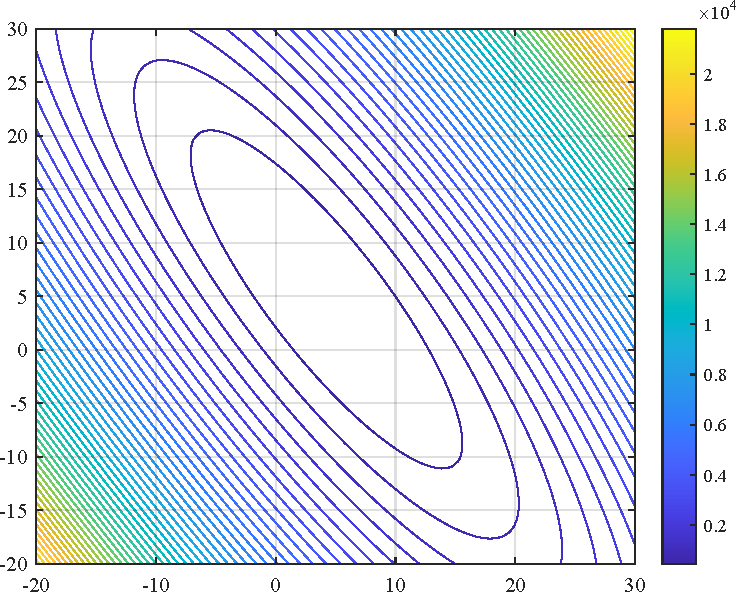
\includegraphics[width=\textwidth]{../Problem 8/contour_2d.pdf}
		\caption{2D plot of MSE index}
		\label{fig:prob_8_2d}
	\end{subfigure}
	\hspace{2mm}
	\begin{subfigure}{0.47\textwidth}
		\centering
		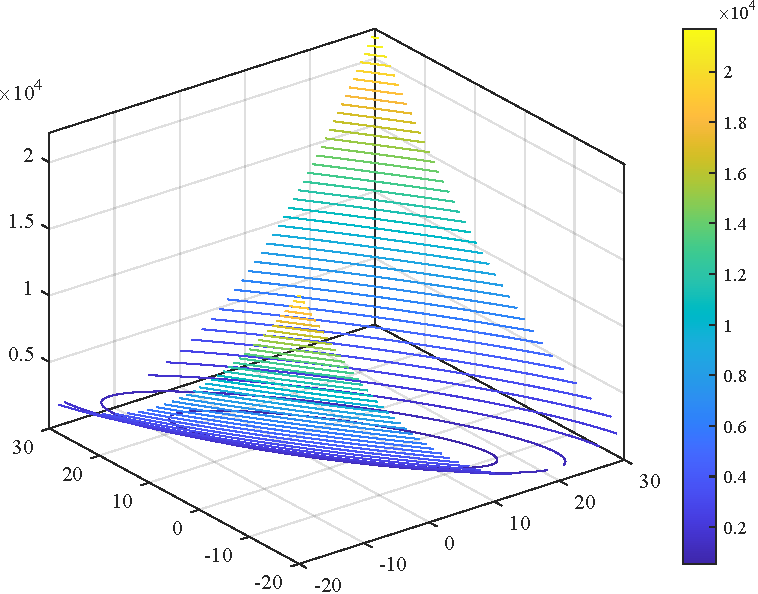
\includegraphics[width=\textwidth]{../Problem 8/contour_3d.pdf}
		\caption{3D plot of MSE index}
		\label{fig:prob_8_3d}
	\end{subfigure}	
\end{figure}

\vspace{2cm}
\subsection{Question c}
A decision boundary is a hypersurface that separates different classes in a classification problem.\\
The optimal decision boundary is the one that minimizes a certain transfer function. Here it is a line that can be described by the equation 
\[
\begin{gathered}
	f(x) = W^T \cdot x^*, 
\end{gathered}
\]
where $
W=\left[\begin{array}{cc}
	W_{11} & W_{12}
\end{array}
\right]
$ and $x^*$ the minimum square error \\
$x^*$ is the strong minimum, a stationary point that is indeed the center of the cycle of Figure \ref{fig:prob_8_2d}.\\

So, in order to find the optimal decision boundary we follow the mentioned steps:
\begin{itemize}
	\item $f(x) = W^T \cdot x^*$
	\item Set f(x) = 0
	\item Calculate $x^* = R^-1 \cdot h$
	\item Replace the value in f(x)
\end{itemize}

By calculating $x^* = R^-1 \cdot h$ we get that $x^* = \left[\begin{array}{c}
															4.2370 \\
															4.7185 \\
														\end{array}
														\right] $

\vspace{5mm}
and the optimal decision boundary is $f(W_{11},W_{12}) = 4.2370 \cdot W_{11} + 4.7185 \cdot W_{12} $ \\

With the help of Matlab we get the following figure \ref{fig:patterns}

\begin{figure}[H]
	\centering
	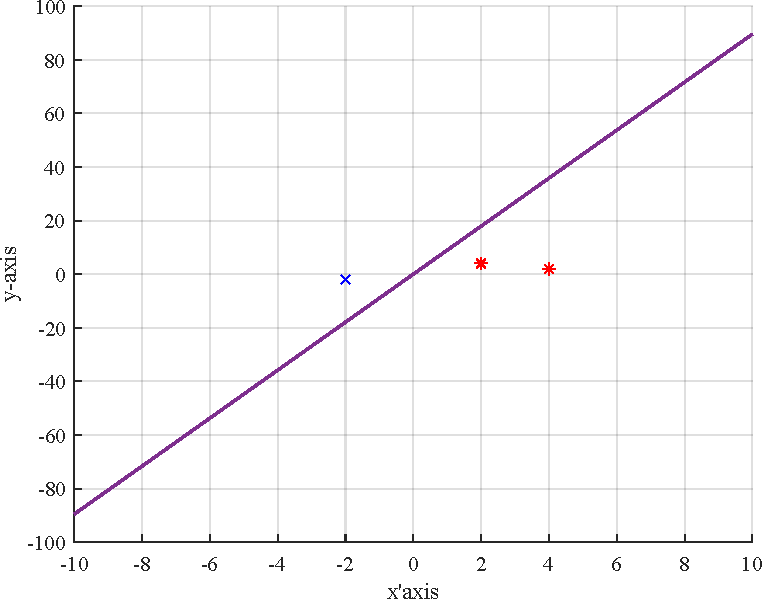
\includegraphics[width = 0.6\textwidth]{../Problem 8/patterns.pdf}
	\caption{Optimal Decision Boundary line and the patterns}
	\label{fig:patterns}
\end{figure}

From the figure \ref{fig:patterns} it is obvious that the optimal decision boundary separates and correctly classifies the patterns. For a binary classification problem,as in our case, all points(\color{red}{*}\color{black}) on one side of the decision boundary are predicted to belong to one class, while points (\color{blue}{x}\color{black}) on the other side are predicted to belong to the other class.\\

\subsection{Question d}
The maximum stable learning rate for the LMS algorithm can be calculated by
$lr_{max} = \dfrac{1}{\lambda_{max}}$ , where ${\lambda_{max}}$ is the largest eigenvalue of the correlation matrix R. With the help of matlab i calculated and found that the eigenvalue matrix of R is 

 \[
 eigenvalue = \left[
\begin{array}{c}  
	1.2293 \\
	17.5707  
\end{array}
\right]
\]
Thus the largest eigenvalue is ${\lambda_{max}} = 17.5707$ and in conclusion the maximum learning rate is $lr_{max} = \dfrac{1}{17.5707}$ $\rightarrow$ \fbox{$lr_{max} = 0.0569$}
\\

As we have already mentioned, the learning rate is related to the correlation matrix R. The matrix R depends only on the properties of the input data -$R = E[p \cdot p^T]$ - and not on the output. The learning rate does not depend on the target values but on the properties of the input data.\\
This means that, changing the target values could potentially affect the convergence of the LMS algorithm and the final solution.However, the maximum stable learning rate itself, as a parameter of the algorithm, would not be directly affected by changes in the target values.\\

\vspace{2mm}

\subsection{Question e}
To perform one iteration of the LMS algorithm we will need a learning rate, the initial weight values and an input. It is given that
\begin{itemize}
	\item Input data: pattern $p_1 = \left[
	\begin{array}{c}
		2 \\
		4
	\end{array}
	\right]
	$
	\item $w(0) = \left[
	\begin{array}{c}
		0 \\
		0
	\end{array}
	\right]
	$
	\item Learning rate: lr = 0.05
\end{itemize}
For a single-layer ADALINE network we recall the rule
\begin{center}
	$W_{k+1} = W_k + 2 \cdot lr \cdot e_k \cdot p_k^T$
\end{center}
where $e_k$ is the error on that step.\\

To begin with, we must follow these steps for the iterations. For k=0 we get:
\begin{itemize}
	\item Step1: Find output $a_k$\\
	$a_0 = purelin(W(0) \cdot p_1) = purelin(w(0) = \left[
	\begin{array}{c}
		0 \\
		0
	\end{array}
	\right] \cdot \left[\begin{array}{c}
		2 \\
		4
	\end{array}
	\right] = 0 $
	\item Step2: Calculate error $e_k$\\
	$e_0 = t_0 - a_0 = t_1 - a_0 = 26 - 0 = 26$
	\item Step3: Calculate weight $W_{k+1}$\\
	$W_{1} = W_0 + 2 \cdot lr \cdot e_0 \cdot p_0^T = w(0) = \left[
	\begin{array}{c}
		0 \\
		0
	\end{array}
	\right] + 2 \cdot 0.05 \cdot e_0 \cdot  \left[
	\begin{array}{c}
		2 \\
		4
	\end{array}
	\right] =  \left[
	\begin{array}{c}
		2 \\
		4
	\end{array}
	\right] =  \left[
	\begin{array}{cc}
		5.2000 & 10.4000 \\
	\end{array}
	\right]$
	
\end{itemize}







	

